\documentclass[a4paper,twoside]{scrbook}
\usepackage{subfigure}
\usepackage[graphicx]{realboxes}
\begin{document}
\title{Volume 1, Part B: Early Supercomputer}
\author{EDI}
\frontmatter
\maketitle
\tableofcontents
\mainmatter

\chapter{Introduction}

what supercomputer architectures have we attempted?

1.Grid computing
在2001年,论文\textbf{The Anatomy of the Grid}作为网格技术领域的奠基性文章,认为网格是为了解决动态、跨机构的虚拟组织中资源共享与协调的问题而提出的。具体来说重新定义网格计算为一种在分布式、高性能计算环境中支持大规模资源共享、协作和虚拟组织(VO)的技术,其关注的是动态集合中的个人、机构和资源之间的灵活、安全和协调的资源共享。并通过协议、服务、API 和SDK 的有机结合,提出一种能够灵活、安全地实现跨机构的资源共享的可扩展的网格架构。论文详细描述了网格架构的要求和框架,在结构层,网格提供对不同资源类型的访问,例如计算、存储和网络资源、代码存储库等。网格通常依赖于现有的结构组件,例如本地资源管理器;连接层定义了核心通信和身份验证协议,以实现简单安全的网络交换;资源层管理资源的使用,包括资源的发布、发现和分配;集合层捕获资源集合之间的交互,支持虚拟组织的创建和管理,协调不同参与者之间的资源共享和协作;应用层包括建立在上述协议和 API 之上并在VO环境中运行的任何用户应用程序。由于网格技术侧重于动态的跨组织共享,因此它与现有的分布式计算技术是互补而非竞争关系。

在2003年,论文\textbf{The Physiology of the Grid}相比于前文则侧重讨论网格机制如何实现面向服务的体系结构,解释了如何将网格功能合并到Web服务框架中。详细的说,论文关注的是响应协议消息的服务的性质,也就是将网格定义为一组可扩展的网格服务,这些服务可以通过各种方式聚合以满足VO的需求,而VO本身可以部分由它们运营和共享的服务来定义。为了实现这样的功能,论文提出了一个开放网格服务架构(OGSA)的概念,OSGA基于网格和Web服务的概念和技术,定义了统一公开的服务语义,OSGA还定义用于创建、命名和发现瞬态网格服务实例的标准机制,为服务实例提供位置透明度和多种协议绑定,并支持与底层原生平台设施集成。OSGA还根据 Web 服务描述语言(WSDL)接口和相关约定定义了创建和组合复杂分布式系统所需的机制,包括生存期管理、变更管理和通知。

在2008年,\textbf{Cloud Computing and Grid Computing 360-Degree Compared}系统性的总结了云计算与网格计算近些年的成果,并深入对比了这两个概念。论文首先定义云计算为一种由规模经济驱动的大规模分布式计算范式,有四个特点:1)它是可大规模扩展的,2)可以封装为一个抽象实体,向云外部的客户提供不同级别的服务,3)它是由规模经济驱动的,4)服务可以动态配置(通过虚拟化或其他方法)并按需交付。云计算是从网格计算演变而来的,并依赖于网格计算的基础设施。作者还指出,尽管云计算和网格计算有许多共同点,但云计算更注重经济性,提供更抽象的资源和服务。在论文的第二部分,作者分别从六个方面:商业模型、结构、资源管理、编程模型、业务模型、安全性上进行更加深入的对比,并认为需要定义协议,允许用户和服务提供商发现需求并将其移交给其他提供商,监控和管理他们的预订,并安排付款,也需要用于管理底层资源和由此产生的分布式计算的工具。
\begin{figure}
\centering %表示居中
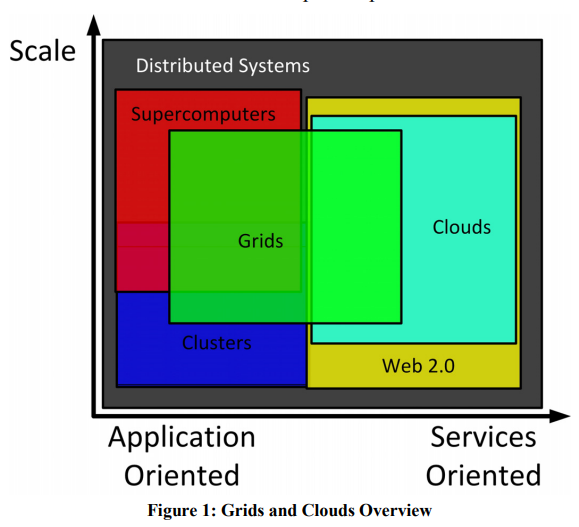
\includegraphics[height=4.5cm,width=9.5cm]{compared.png}
\caption{pic1}
\end{figure}


2.Cloud Computing
在2009年,论文\textbf{A View of Cloud Computing}认为云计算既指通过互联网作为服务交付的应用程序,也指提供这些服务的数据中心中的硬件和系统软件。云计算包括通过互联网提供的应用服务(SaaS)和支持这些服务的基础设施和平台。论文讨论了公共云和私有云的区别,并提出了云计算的三个主要创新点:按需提供无限计算资源;消除用户的前期投入;根据短期需求按使用量付费。论文认为云计算面临10大机遇与挑战,如下图所示。其中业务连续性和服务可用性、数据锁定、数据机密性这三个影响云计算的采用效果,数据传输瓶颈、性能不可预测性、可扩展存储、调试和故障排除、规模快速扩展这五个影响云计算的发展情况,最后软件许可和声誉和服务水平协议这两个是政策和业务方面的问题。此外,云计算的计算、存储和网络都必须关注虚拟化资源的水平可扩展性,而不是单节点性能。
\begin{figure}
\centering %表示居中
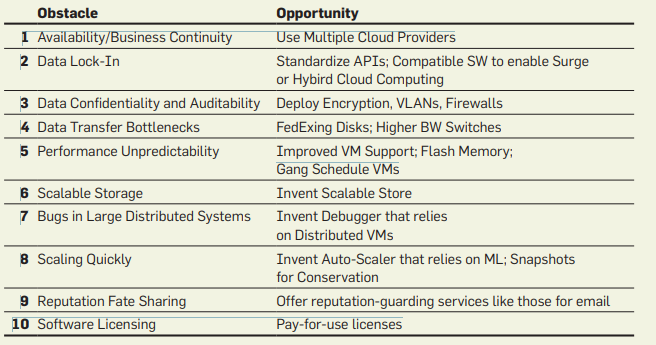
\includegraphics[height=4.5cm,width=9.5cm]{cloud10.png}
\caption{pic2}
\end{figure}

在2010年,论文\textbf{Cloud computing: state-of-the-art and research challenges}介绍了云计算的兴起背景及其对IT行业的影响。云计算通过按需提供计算资源,为企业节省成本,并提供了高度的可扩展性和易访问性。
论文再次提出,网格计算是一种分布式计算范式,它协调网络资源以实现共同的计算目标。云计算与网格计算类似,因为它也使用分布式资源来实现应用程序级目标。然而,云计算更进一步,通过利用多层次(硬件和应用平台)的虚拟化技术来实现资源共享和动态资源供应。云计算具有按需自助服务、广泛的网络访问、资源池化、快速弹性、衡量服务等特性。
云计算环境的架构通常可以分为四个层次:硬件/数据中心层、基础设施层、平台层和应用层。硬件层负责管理云计算的物理资源,包括物理服务器、路由器、交换机、电力和冷却系统。基础设施层又称虚拟化层,通过利用虚拟化技术对物理资源进行分区,创建一个存储和计算资源池。在基础设施层之上,平台层包括操作系统和应用框架。平台层的目的是最小化将应用程序直接部署到虚拟机容器中的负担。在应用层中,云计算的架构与传统的服务托管环境相比更加模块化。每一层与上下层之间耦合松散,使每一层能够独立发展。这类似于OSI 网络协议模型的设计。

在2011年,美国国家标准与技术研究院在论文\textbf{The NIST Definition of Cloud  Computing}中对不断发展的云计算概念作出定义,并总结之前的研究明确了几个特征。云计算是一种模型,旨在通过网络方便地按需访问可配置计算资源的共享池,如网络、服务器、存储、应用程序和服务。这些资源可以快速配置和发布,只需最少的管理工作或服务提供商交互。包含五个基本特征,三种服务模型,四种部署模型。
\textbf{五个基本特征}
按需自助服务 :消费者可以根据需要自动配置计算能力(如服务器时间和网络存储),无需与每个服务提供者互动。
广泛的网络访问 :功能通过网络提供,并通过标准机制访问,支持各种客户端平台(如移动电话、平板电脑、笔记本电脑和工作站)。
资源池化:提供者的计算资源被池化以服务多个消费者,采用多租户模型,资源根据需求动态分配和重新分配,消费者对资源的确切位置没有控制权。
快速弹性 :能力可以快速扩展和收缩,以适应需求,消费者认为这些能力是无限的,并且可以在任何时间以任何数量使用。
测量服务:云系统自动控制和优化资源使用,通过适当的抽象层级进行计量,提供透明的资源使用情况。
\textbf{三种服务模型}
软件即服务:消费者使用提供者运行在云基础设施上的应用程序,通常通过网络浏览器或程序接口访问,消费者不管理或控制底层云基础设施。
平台即服务:消费者在云基础设施上部署自制或获取的应用程序,使用提供者支持的编程语言、库、服务和工具,消费者不管理底层云基础设施。
基础设施即服务:消费者可以配置处理、存储、网络等基础计算资源,能够部署和运行任意软件,包括操作系统和应用程序,消费者对底层云基础设施没有管理权,但可以控制操作系统、存储和部署的应用程序。
\textbf{四种部署模型}
私有云 :为单一组织专用,可能由组织、第三方或两者的组合管理和操作,可以在场内或场外存在。
社区云 :为特定社区的消费者专用,共享关切(如任务、安全要求、政策和合规考虑),可能由一个或多个社区组织、第三方或两者的组合管理和操作。
公共云:为公众开放使用,可能由商业、学术或政府组织管理和操作,存在于云提供者的场所。
混合云:由两个或多个不同的云基础设施(私有云、社区云或公共云)组成,通过标准化或专有技术绑定在一起,支持数据和应用程序的可移植性。

在2011年,论文\textbf{Cluster, Grid and Cloud Computing: A Detailed Comparison}介绍高性能计算曾经是专属于能够负担昂贵专用超级计算机的机构。随着小规模、低成本高性能计算需求的增加,集群计算应运而生。网格计算在1990年代中期起源于学术界,旨在允许用户远程利用其他计算中心的闲置计算资源。云计算则在2007年底出现,提供了用户可以通过互联网访问的计算资源池,核心原则是将计算从本地计算机转移到网络上,以减少企业在硬件和软件上的投资。集群计算是由一组并行或分布式计算机组成,通过高速网络互联,协同执行计算密集型和数据密集型任务。集群计算主要用于高可用性、负载均衡和计算目的,通过维护冗余节点来提高系统的可靠性和性能。网格计算结合来自多个管理域的计算机以实现共同目标,解决单一任务,可以迅速消失。网格计算的主要策略是使用中间件将程序分成若干部分,并分配到不同计算机。云计算指通过互联网提供的应用和提供这些服务的数据中心的硬件和系统软件。论文还介绍了这几种方式所面临的挑战,随后论文从多方面比较了这三种计算,如下图所示:
\begin{figure}
\centering %表示居中
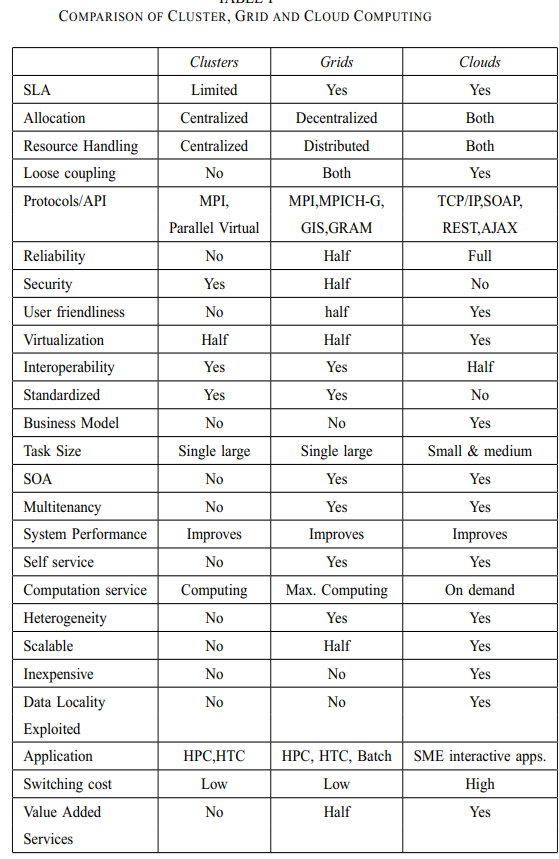
\includegraphics[height=12.5cm,width=9.5cm]{c c g compaerd.png}
\caption{pic3}
\end{figure}
可以看出,在我们之前整理的虚拟化、资源分配等方面做出了清晰的对比。
3.Edge/fog computing
在2012年,论文\textbf{Fog Computing and Its Role in the Internet of Things}探讨了雾计算的概念及其在物联网中的应用。雾计算扩展了云计算的范式,将其延伸到网络边缘,从而支持一类新的应用和服务。雾计算的定义特征包括a)低延迟和位置感知,b)地理分布广泛,c)流动性,d)节点数量非常多,e)无线接入的主导作用,f)流和实时应用程序的强大存在,g)异构性。论文认为这些特征使雾计算成为支持一些关键物联网服务和应用(的适当平台。新兴的互联网部署浪潮,尤其是物联网,除了位置感知和低延迟外,还需要移动支持和地理分布。论文认为需要一个新的平台来满足这些要求,即雾计算。或者简单地说,雾,仅仅是因为雾是靠近地面的云。而网络边缘的主要特点是其地理位置靠近数据生成源,从而能够提供更低的延迟、更高的带宽效率和更即时的数据处理能力。
雾计算节点通常部署在网络边缘,靠近数据生成源,从而能够提供更低的延迟和更高的位置感知。这对于需要实时处理的应用(如游戏、视频流、增强现实等)特别重要。

在2016年,论文\textbf{Edge Computing: Vision and Challenges}介绍到,边缘计算是指允许在网络边缘、代表云服务的下游数据和代表物联网服务的上游数据执行计算的使能技术。边缘计算更侧重于事物方面,而雾计算更侧重于基础设施方面。边缘计算可以在智能环境领域蓬勃发展,例如,智慧城市中,大量传感器和设备生成的数据可以在边缘节点进行处理,例如交通管理、环境监测和公共安全。通过在靠近数据源的地方进行处理,可以减少延迟,提供更及时的响应,并减少带宽需求;在智慧照明系统中,可以在本地处理传感器数据,以根据实时情况调整照明强度,从而提高能源效率和用户体验。论文还引入了协作边缘,因为边缘可以在物理和逻辑上连接最终用户和云,因此不仅仍然支持传统的云计算范式,而且由于数据的紧密性,它可以将远距离网络连接在一起进行数据共享和协作。

在2020年,论文\textbf{An Overview on Edge Computing Research}介绍到,中国边缘计算产业联盟将边缘计算定义为在网络或数据源边缘提供核心能力的开放平台,满足行业在连接、实时业务、数据优化、应用智能、安全和隐私方面的关键需求。如今,随着物联网在人们生活中的普及和发展,连接到物联网的设备数量逐渐增加,并产生了大量的数据。云计算的网络带宽已经无法满足时间敏感系统和实时性能的需求,因此,云计算模型在负载、实时性、传输带宽、能耗以及数据安全和隐私保护方面存在较大缺陷。
\begin{figure}
\centering %表示居中
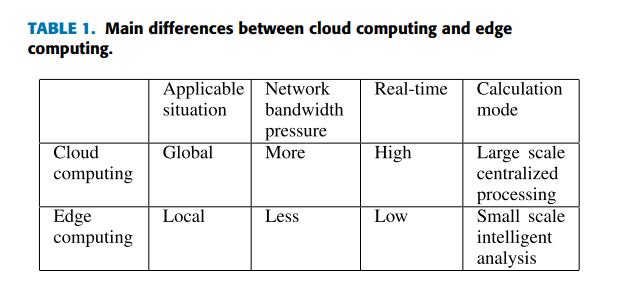
\includegraphics[height=4.5cm,width=9.5cm]{edge1.png}
\caption{pic4}
\end{figure}
针对边缘计算的结构,论文给出如下部分:边缘设备是边缘计算体系结构的基础组成部分,通常具有一定的计算和存储能力,可以在本地执行数据处理任务,从而减少对云端计算资源的依赖;边缘节点是位于边缘设备和云计算中心之间的中间层,这些节点具有更强的计算和存储能力,可以在本地完成复杂的数据处理任务,从而提高响应速度和数据处理效率;边缘网关是连接边缘设备和边缘节点的关键组件。它们负责数据的收集、过滤和传输,以及不同网络协议之间的转换;尽管边缘计算强调在本地处理数据,但云计算仍然在整个体系结构中扮演重要角色。云计算中心负责存储和处理大量数据,并提供强大的计算和分析能力;高速、低延迟的通信网络能够确保数据在不同组件之间的快速传输。

4.Pervasive Computing
早在2001年,论文\textbf{Pervasive Computing:Vision and Challenges}首先探讨普适计算与其前身(分布式系统和移动计算)的关系,并认为普适计算环境是一个充满计算和通信能力的环境,与用户和谐集成。然后确定了四个新的研究方向:智能空间的有效利用:通过将计算基础设施嵌入建筑基础设施中,智能空间将两个以前不相关的世界结合在一起。这种融合使一个世界可以感知和控制另一个世界。隐形化:理想的状态是普适计算技术完全从用户的意识中消失。本地化:可扩展性随着智能空间的复杂化,用户的个人计算空间与周围环境的互动强度增加,这对带宽、能量都有严重影响。掩盖不均匀的条件:普适计算技术的渗透速率会因非技术因素而变化很大。为了减少用户感受到的变化,可以让个人计算空间弥补“哑”环境的不足。

在2003年,论文\textbf{Pervasive Computing: A Paradigm for the 21st Century}认为普适计算是指计算技术无处不在、融入日常生活的计算模式。Mark Weiser在1991年提出了这一构想,他认为“最深刻的技术是那些消失于无形的技术”,即这些技术会自然地融入我们的日常生活。分布式计算通过引入对远程信息资源的无缝访问以及具有容错、高可用性和安全性的通信,标志着普适计算的演进;移动计算的“随时随地”目标本质上是一种被动的信息访问方法,但它为普适计算的主动“随时随地”目标铺平了道路。构建无处不在的计算环境所需的技术进步分为四大领域:设备:智能环境可能包含多种设备类型,如传统输入设备、无线移动设备和智能设备。网络:未来几年普适设备数量将迅速增长,需要改造现有技术以应对需求,并将这些设备完全整合到现有社会系统中。中间件:需要一个中间件“壳”来在网络内核和用户应用之间进行接口。中间件将主要由固件和软件包组成,以客户端-服务器或对等模式执行。应用程序:普适计算更注重环境,因此应用程序将很大程度上指导中间件和网络问题。

\end{document}
